% Domainanalyse

\section{Domainanalyse}
\label{sec:Domainanalyse}

\begin{figure}[H]
	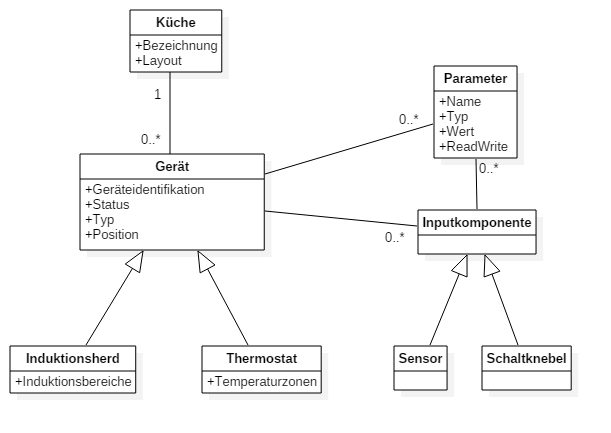
\includegraphics[scale=0.6]{analysis/res/Domain}
	\caption{Domainanalyse \enquote{Küche mit Geräten und Parametern}}
\end{figure}


\subsection{Kurzbeschreibung der Begriffe}
\label{subsec:Kurzbeschreibung der Begriffe}

\subsubsection{Küche}
\label{subsubsec:Küche}
Eine Küche ist im Kontext dieser Applikation \enquote{nur} eine Ansammlung von Geräten mir ihrer Positionierung. Als Layout einer Küche werden die Gegebenheiten vor Ort bezeichnet. Dies kann z.B. ein Grundriss oder ein Foto der Küche sein. Dabei werden nur die wesentlichen Elemente betrachtet, d.h. keine Spülbecken oder Abfalleimer.

\subsubsection{Gerät}
\label{subsubsec:Gerät}
Ein Gerät wird über seine Geräteidentifikation (ID) identifiziert. Es hat einen Status und einen Typ. Zudem ist sein Einbauort in der Küche für den Benutzer wichtig.

\subsubsection{Parameter}
\label{subsubsec:Parameter}
Die Gerätekonfiguration besteht aus einer Liste von Parametern. Diese unterscheiden sich durch ihren Namen und ihren Datentyp. Zudem gibt es Parameter, welche nur ausgelesen, aber nicht verändert werden können.

\subsubsection{Induktionsherd}
\label{subsubsec:Induktionsherd}
Induktionsherde erhitzen das Kochgut mittels elektromagnetischen Effekten. Dabei wird über eine Spule ein Magnetfeld erzeugt, welches die Pfanne oder den Topf direkt anregt und somit erhitzt.

Diese Kochmodule haben Temperaturfühler und eine Topferkennung. Bei der Erkennung wird sichergestellt, dass die Leistungsabgabe nur erfolgt, wenn auch ein gefüllter Topf auf der Oberfläche steht.

Die Firma Fluxron vertreibt verschiedene Modelle von Induktionsgeräten, diese unterscheiden sich in deren Funktionalität. Einige Modelle bieten unterschiedlich Steuerbare Kochzonen, andere haben eine höhenverstellbare Spule für einen flexibleren Einbau.

\subsubsection{Thermostat}
\label{subsubsec:Thermostat}

Die Thermostaten werden meist in andere Geräte, wie z.B. einen Kontaktgrill, verbaut. Dabei messen Sie die Temperatur der Heizfläche und geben den Heizstrom frei oder unterbrechen ihn. Auch hier gibt es verschiedene Varianten mit einer unterschiedlichen Anzahl von Heizzonen (Solltemperatur + Regelausgang).

\subsubsection{Inputkomponente}
\label{subsubsec:Inputkomponente}

Inputkomponenten lesen externe Werte ein. Dies kann z.B. ein Temperatursensor oder ein Schaltknebel (Drehknopf) sein. Die Sensoren und Schaltknebel werden im Hintergrund ebenfalls als set von Parametern abgebildet.